\documentclass[11pt,a4paper]{article}
\usepackage[margin=20mm,headheight=14pt,footskip=10mm]{geometry}
\usepackage[T1]{fontenc}
\usepackage{lmodern,microtype,amsmath,amssymb,booktabs,tabularx,graphicx,xcolor}
\usepackage{fancyhdr}
\usepackage[colorlinks=true,linkcolor=blue!55!black,urlcolor=blue!55!black]{hyperref}
\hypersetup{pdftitle={Envelope and quadratic detection in temporal interference},pdfauthor={TN0484 working note}}
\setlength{\parindent}{0pt}
\setlength{\parskip}{5pt}
\setlength{\abovedisplayskip}{6pt}
\setlength{\belowdisplayskip}{6pt}
\pagestyle{fancy}\fancyhf{}
\fancyfoot[L]{\small TN0484 / WP0185\quad Reading note, October 6, 2026}
\fancyfoot[R]{\small\thepage}
\renewcommand{\headrulewidth}{0pt}
\newcommand{\xx}{\mathbf{x}}
\newcommand{\head}[1]{\par\vspace{4pt}{\large\bfseries #1}\par\vspace{2pt}}
\newcommand{\avg}[1]{\left\langle #1\right\rangle}
\begin{document}
{\LARGE\bfseries Envelope and quadratic detection\\in temporal interference}\par
\vspace{3pt}
Both descriptions start from the same two-tone field. Grossman's focality map uses
envelope excursion; our quadratic detector responds to the squared envelope.
The applied field has no DC component. Both an ideal
envelope follower and a quadratic detector have a nonzero mean output, but their
modulation maps differ. An envelope map alone does not specify a neuron's mean response.

\head{The amplitudes are spatial fields}
Let $\xx$ denote position, $t$ time, and $\omega_1,\omega_2$ two nearby carrier angular
frequencies, with beat frequency $\Omega=|\omega_1-\omega_2|$. For a fixed polarization
direction, write the membrane input as
\begin{equation}
u(\xx,t)=a(\xx)\cos\omega_1t+b(\xx)\cos\omega_2t .
\label{eq:input}
\end{equation}
Here $a(\xx)$ and $b(\xx)$ are signed local polarization amplitudes, including linear
field-to-membrane access. They vary in space and are held fixed only while averaging
over time at one location. The positive envelope is
\begin{equation}
A(\xx,t)=\sqrt{a(\xx)^2+b(\xx)^2+2a(\xx)b(\xx)\cos\Omega t}.
\label{eq:envelope}
\end{equation}
The conventional TI map is the envelope's temporal excursion, $\max_t A-\min_t A$,
projected along the chosen direction~[1]. An ideal envelope-following response is
$y_{\rm env}=k_1 A$, with constant gain $k_1>0$; this is a comparator, not a cellular
transfer function established by Grossman et al.

\head{The detector sets the mean and modulation maps}
For a smooth static transfer $g$ about baseline $v_*$, define
$k_2=g''(v_*)/2\ne0$. To second order, the carrier-averaged response change is
$y_{\rm quad}=k_2 P$, where
\begin{equation}
P(\xx,t)=\frac{A(\xx,t)^2}{2}
=\frac{a(\xx)^2+b(\xx)^2}{2}+a(\xx)b(\xx)\cos\Omega t .
\label{eq:power}
\end{equation}
Carrier averaging removes the fast lines but retains the beat; averaging over a
beat period then gives the DC component. The table compares the geometric maps
before multiplying by $k_1$ or $k_2$. Their units differ, so spatial contrasts,
not absolute magnitudes, are comparable.

\begin{center}
\renewcommand{\arraystretch}{1.45}
\begin{tabularx}{\textwidth}{@{}p{0.22\textwidth}XX@{}}
\toprule
 & \textbf{Envelope following} & \textbf{Quadratic detection}\\
\midrule
Slow signal & $A(\xx,t)$ & $P(\xx,t)=A(\xx,t)^2/2$\\
Mean (DC) & $D_{\rm env}(\xx)=\overline A(\xx)$
 & $D_{\rm quad}(\xx)=\dfrac{a(\xx)^2+b(\xx)^2}{2}$\\
Modulation\newline(max--min) & $M_{\rm env}(\xx)=2\min(|a(\xx)|,|b(\xx)|)$
 & $M_{\rm quad}(\xx)=2|a(\xx)b(\xx)|$\\
\bottomrule
\end{tabularx}
\end{center}
Here $\overline A(\xx)=(2\pi)^{-1}\int_0^{2\pi}
\sqrt{a(\xx)^2+b(\xx)^2+2a(\xx)b(\xx)\cos\theta}\,d\theta$, with $\theta$ the beat phase.
For matched amplitudes $a(\xx)=b(\xx)=s>0$ at a site, the means are $4s/\pi$ and $s^2$,
respectively. A nonzero envelope mean is not a DC electric field. It becomes a mean
detector output only under the envelope-following assumption; adaptation may remove it.
The quadratic mean is a signed response change after multiplication by $k_2$.
Even a single carrier ($b=0$) gives both ideal detectors a mean output,
but no beat modulation.

\vfill
{\footnotesize [1] Grossman et al., \emph{Cell} \textbf{169}, 1029--1041.e16 (2017),
Figs.~1--2 and STAR Methods.
\href{https://doi.org/10.1016/j.cell.2017.05.024}{doi:10.1016/j.cell.2017.05.024}.
The scalar comparison fixes a direction; maximizing over directions is a separate operation.}

\newpage
\head{The two modulation maps can rank locations differently}
The relation is pointwise:
\begin{equation}
M_{\rm quad}(\xx)=\max(|a(\xx)|,|b(\xx)|)\,M_{\rm env}(\xx).
\label{eq:reweight}
\end{equation}
The quadratic map weights the conventional envelope map by the stronger local
carrier. Thus an envelope focus need not remain the strongest quadratic response.
The example below also shows that quadratic detection can retain a central modulation peak.

\begin{center}
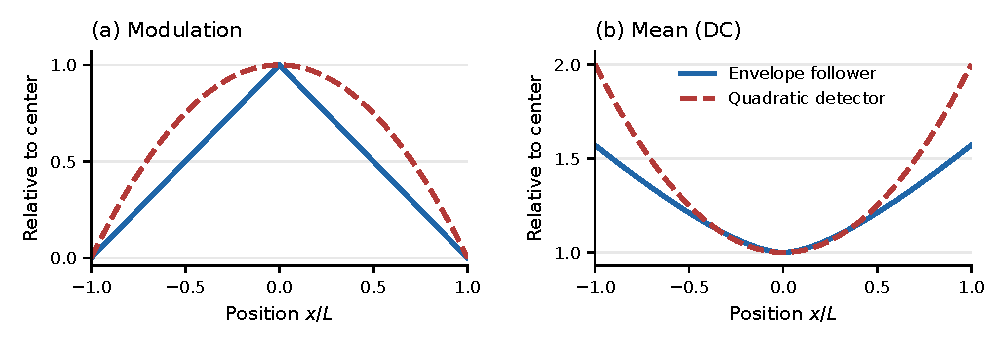
\includegraphics[width=\textwidth]{spatial_maps.pdf}
\end{center}
{\small\textbf{Figure 1.} Illustrative line profile:
$a(x)=a_0(1+x/L)$ and $b(x)=a_0(1-x/L)$ on $-L\le x\le L$, with polarization scale
$a_0>0$ and length $L>0$. Each curve is divided by its own value at $x=0$.
(a) Modulation is $1-|x/L|$ for envelope following and $1-(x/L)^2$ for quadratic
detection: both peak centrally, but the quadratic profile is broader here.
(b) Both means increase toward the edges. This is a line profile, not a head model
or a demonstration of three-dimensional focusing.}

A separate two-site example shows a reversal. Give a target the amplitudes
$(a,b)=(\epsilon,\epsilon)$ and an off-target site $(10\epsilon,0.2\epsilon)$,
where $\epsilon>0$ sets the polarization scale:
\begin{center}
\renewcommand{\arraystretch}{1.15}
\begin{tabular}{@{}lcc@{}}
\toprule
Modulation map & Target & Off-target\\
\midrule
Envelope excursion & $2\epsilon$ & $0.4\epsilon$\\
Quadratic excursion & $2\epsilon^2$ & $4\epsilon^2$\\
\bottomrule
\end{tabular}
\end{center}
The envelope favors the target fivefold; the quadratic detector favors the off-target
site twofold. These are illustrative amplitudes, not a simulated montage. Reducing
$\epsilon$ preserves these ratios while taking the quadratic detector into its weak-input regime.

\head{A DC restriction does not prohibit a beat focus}
In a source-free, homogeneous isotropic conductor, fixed linear access and orientation
make $a(\xx)$ and $b(\xx)$ harmonic. With $\nabla$ denoting spatial derivatives,
\begin{equation}
\nabla^2D_{\rm quad}=|\nabla a|^2+|\nabla b|^2\ge0,
\qquad
\nabla^2(ab)=2\nabla a\cdot\nabla b .
\end{equation}
The quadratic DC map has no strict interior maximum; the beat product has no such
restriction. The envelope mean $D_{\rm env}$ also has no strict interior maximum:
at each beat phase, $A$ is the norm of a vector of harmonic functions, hence is
subharmonic, and averaging preserves this property. This restriction therefore
applies to both idealized mean maps. Compartment boundaries include tissue interfaces;
the theorem does not locate the maximum at the scalp.

These are local detector maps. A network with linear susceptibility $G_{\xx}(\omega)$
responds differently at DC and at $\Omega$; resonance can favor modulation over a
mean shift. Spatially varying access, curvature, orientation, and network gain require
separate weighting. Dynamic detectors also have frequency-dependent coefficients.
TI selectivity remains possible, but its response map must follow the detector law;
the envelope map alone cannot establish quadratic-response focality.
\end{document}
